% 1964 附加题（2）：正方体内两球的空间示意（矢量重绘）
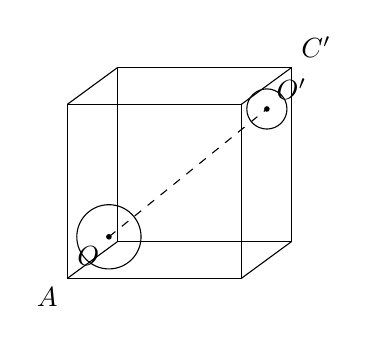
\begin{tikzpicture}[>=stealth,scale=0.85]
  \coordinate (A) at (0,0);
  \coordinate (B) at (2.6,0);
  \coordinate (C) at (2.6,2.6);
  \coordinate (D) at (0,2.6);
  \coordinate (Ap) at (0.75,0.55);
  \coordinate (Bp) at (3.35,0.55);
  \coordinate (Cp) at (3.35,3.15);
  \coordinate (Dp) at (0.75,3.15);
  \draw (A)--(B)--(C)--(D)--cycle;
  \draw (Ap)--(Bp)--(Cp)--(Dp)--cycle;
  \draw (A)--(Ap) (B)--(Bp) (C)--(Cp) (D)--(Dp);
  \draw (0.62,0.62) circle (0.48);
  \draw (2.98,2.53) circle (0.30);
  \fill (0.62,0.62) circle (1.2pt) node[below left] {$O$};
  \fill (2.98,2.53) circle (1.2pt) node[above right] {$O'$};
  \draw[dashed] (0.62,0.62)--(2.98,2.53);
  \node[below left] at (A) {$A$};
  \node[above right] at (Cp) {$C'$};
\end{tikzpicture}
